%Type of document
\documentclass[a4paper, 12pt]{report}

%For easy management of document margins and the document page size
\usepackage[right=2.9cm,left=2.9cm,top=3.5cm,bottom=3.5cm]{geometry}

%Allows to insert graphic files within a document
\usepackage{graphicx}

%Sup­ports com­pressed, sorted lists of nu­mer­i­cal ci­ta­tions, and also deals with var­i­ous punc­tu­a­tion and %other is­sues of rep­re­sen­ta­tion, in­clud­ing com­pre­hen­sive man­age­ment of break points
\usepackage{cite}

%It gives LaTeX the possibility to manage links within the document or to any URL when you compile in PDF
\usepackage{hyperref}

%To choose the font encoding of the output text
\usepackage[T1]{fontenc}

%To choose the encoding of the input text
%Consente di usare le lettere accentate
\usepackage[latin1]{inputenc}

%It provides the internationalization of LaTeX. It has to be loaded in any document, and you have to give %as an option the main language you are going to use in the document
\usepackage[english]{babel}
\usepackage{pdflscape}

%Provides compact, "starred" versions for the lists (itemize) 
\usepackage{mdwlist}

\normalfont
%Forza LaTeX ad una spaziatura uniforme, invece di lasciare più spazio
%alla fine dei punti fermi come da convenzione inglese
\frenchspacing
%Modifica della spaziatura interlineare
\linespread{1.3}

%Inizia il documento
\begin{document}

%Creazione di un frontespizio personalizzato
\begin{titlepage}

\begin{center}
\Large
\textbf{POLYTECHNIC UNIVERSITY OF MILAN} \\
\Large
School of Industrial and Information Engineering \\
Computer Science and Engineering
\end{center}

\addvspace{0.8cm}
%PER INSERIRE IMMAGINE
\begin{figure}[h]
\begin{center}

\includegraphics[width=3cm]{cpt/img/polimi}
\end{center}
\end{figure}

\addvspace{0.1cm}
\begin{center}
\LARGE

\textbf{Project of Software Engineering 2: MyTaxi Service \\
Integration Test Plan Document}

\end{center}

\addvspace{0.5cm}
\Large
\begin{center}
\begin{tabular}{p{1\textwidth}p{0.3\textwidth}}
Course Professor: Prof. Elisabetta DI NITTO \\
\end{tabular}
\end{center}

\addvspace{0.6cm}
\Large
\begin{center}
\begin{tabular}{p{0.6\textwidth}p{0.6\textwidth}}
& Authors: \\
& Mattia 	CRIPPA		854126\\
& Francesca GALLUZZI	788328\\
& Marco 	LATTARULO	841399
\end{tabular}
\end{center}

\vfill
\Large
\begin{center}
Academic Year 2015--2016
\end{center}
\end{titlepage}

\clearpage

\tableofcontents
\clearpage

\chapter{Introduction}
\clearpage

\chapter{Integration Strategy} \label{chap2}

\section{Entry Criteria}
The Integration Testing can be carried out after the successful completion of the Unit Testing of the entire software. In addition the following points should be valid:

\begin{itemize}
	\item The project should be code-complete and all its major features should be already present
	\item The project should satisfy the memory requirements specified in the RASD
	\item The correct version of the software is moved into the integration testing environment
	\item Sanity testing is done and build is stable for further testing
	\item The Database should be ready and its tables are populated with initial data
\end{itemize}

\section{Elements to be Integrated}
Due to the early stage of development of the software and the resulting low level of complexity of the entire system, we decided to focus our integration testing only on the main components of the Business Logic, keeping in mind that the future evolution of the project will lead to the creation of a number of subcomponent inside these component, needed to make the system fully working. Following this decision, we are going to integrate the Web Component and the Business Logic Component, testing the direct connections between the managed Beans and their corresponding Managers and we are also going to integrate the 7 subcomponents of the Business Logic Component.

\section{Integration Testing Strategy}
Due to the particular stage of development explained in the previous point, at the moment there is not a complete hierarchy of (sub)components and (sub)systems, so it?s not possible to fully define the integration test strategy followed in this document, because all the components involved are on the same level. Anyway the selected approach is the top-down approach, because (as stated in the previous point) in the future other lower level subcomponents will be implemented and then the testing will follow this downward development.

\section{Sequence of Component / Function Integration}

\begin{figure}[!htbp]
\centering
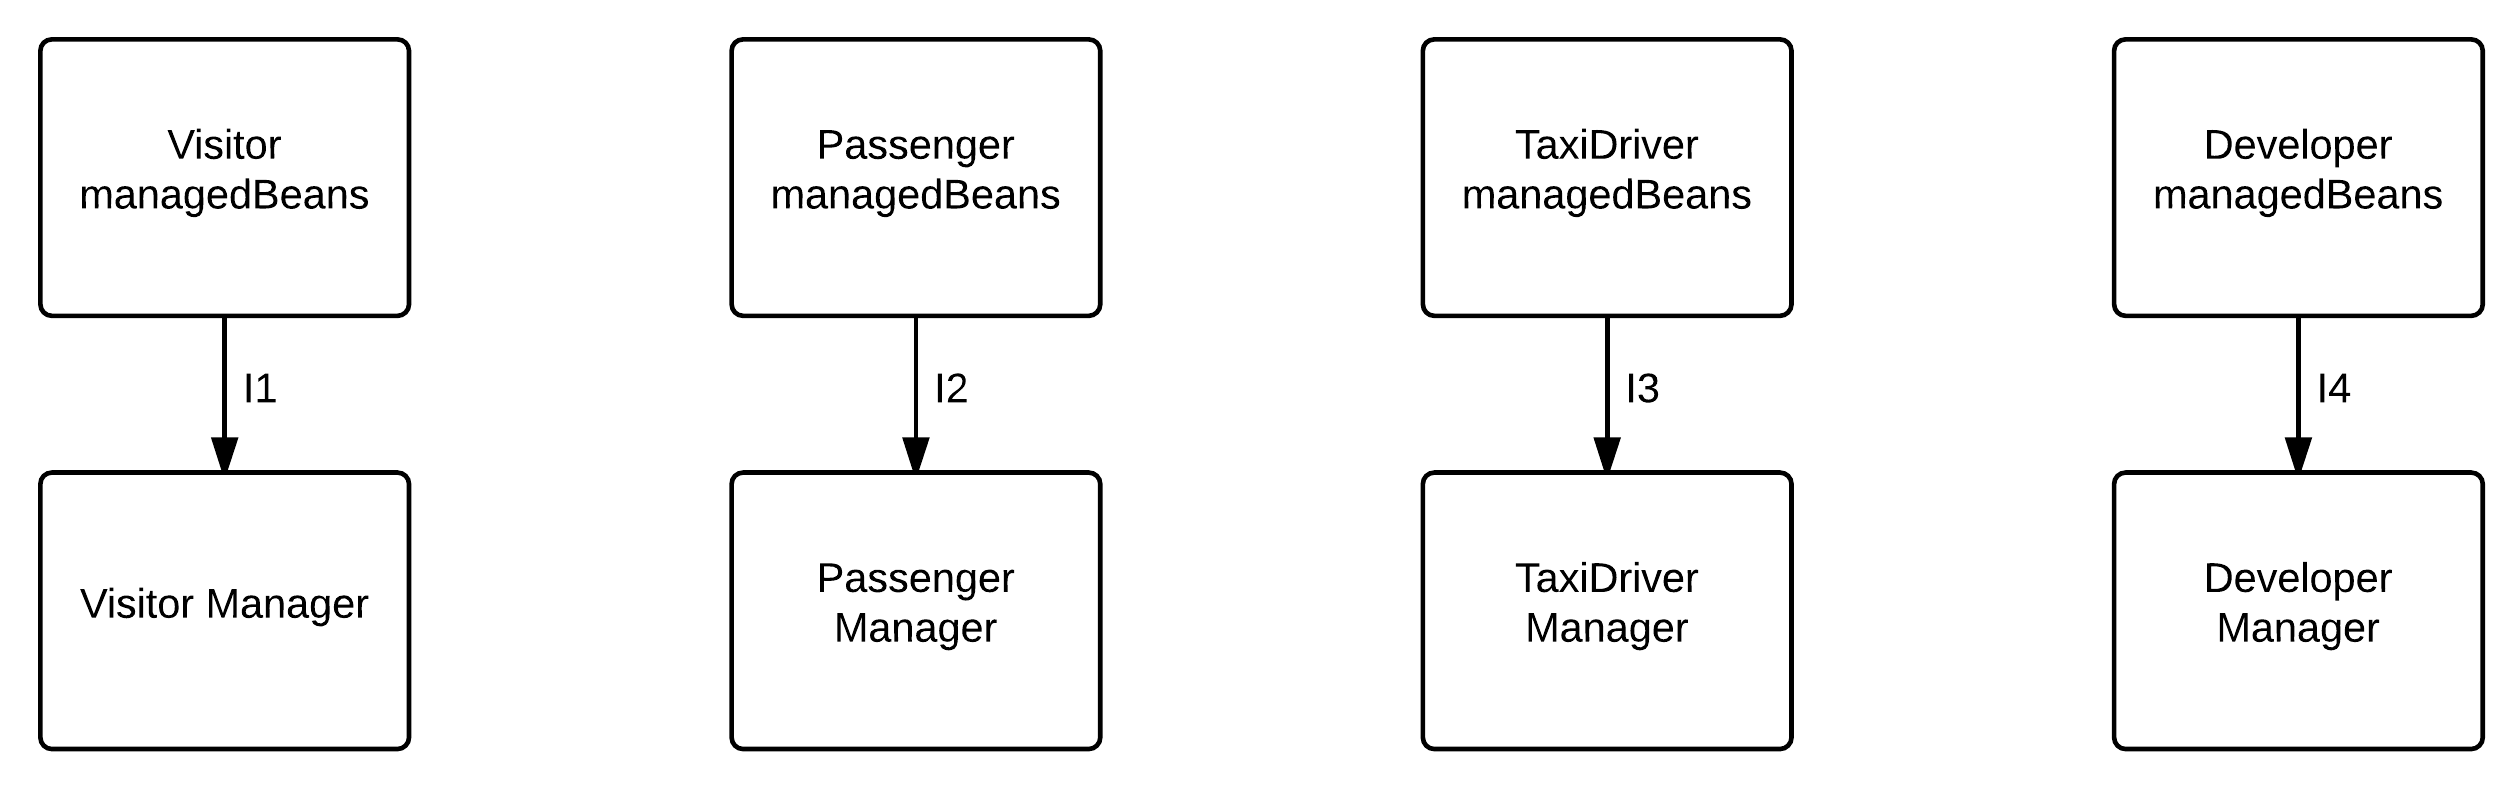
\includegraphics[width=\textwidth]{cpt/img/ITDPComponentDiagramsTP1}
\end{figure}

\begin{table}[!htbp]
\begin{center}
\begin{tabular}[t]{c|p{0.7\textwidth}|c}

\textbf{ID} & \textbf{Integration Test} & \textbf{Paragraphs} \\
\hline
I1 & Visitor managedBean $\rightarrow$ Visitor Manager & 3.1.1  3.2.1 \\
\hline
I2 & Passenger managedBean $\rightarrow$ Passenger Manager & 3.1.2  3.2.1 \\
\hline
I3 & TaxiDriver managedBean $\rightarrow$ TaxiDriver Manager & 3.1.3  3.2.1 \\
\hline
I4 & Developer managedBean $\rightarrow$ Developer Manager & 3.1.4  3.2.1 \\
\hline
\end{tabular}
\end{center}
\end{table}

\begin{figure}[!htbp]
\centering
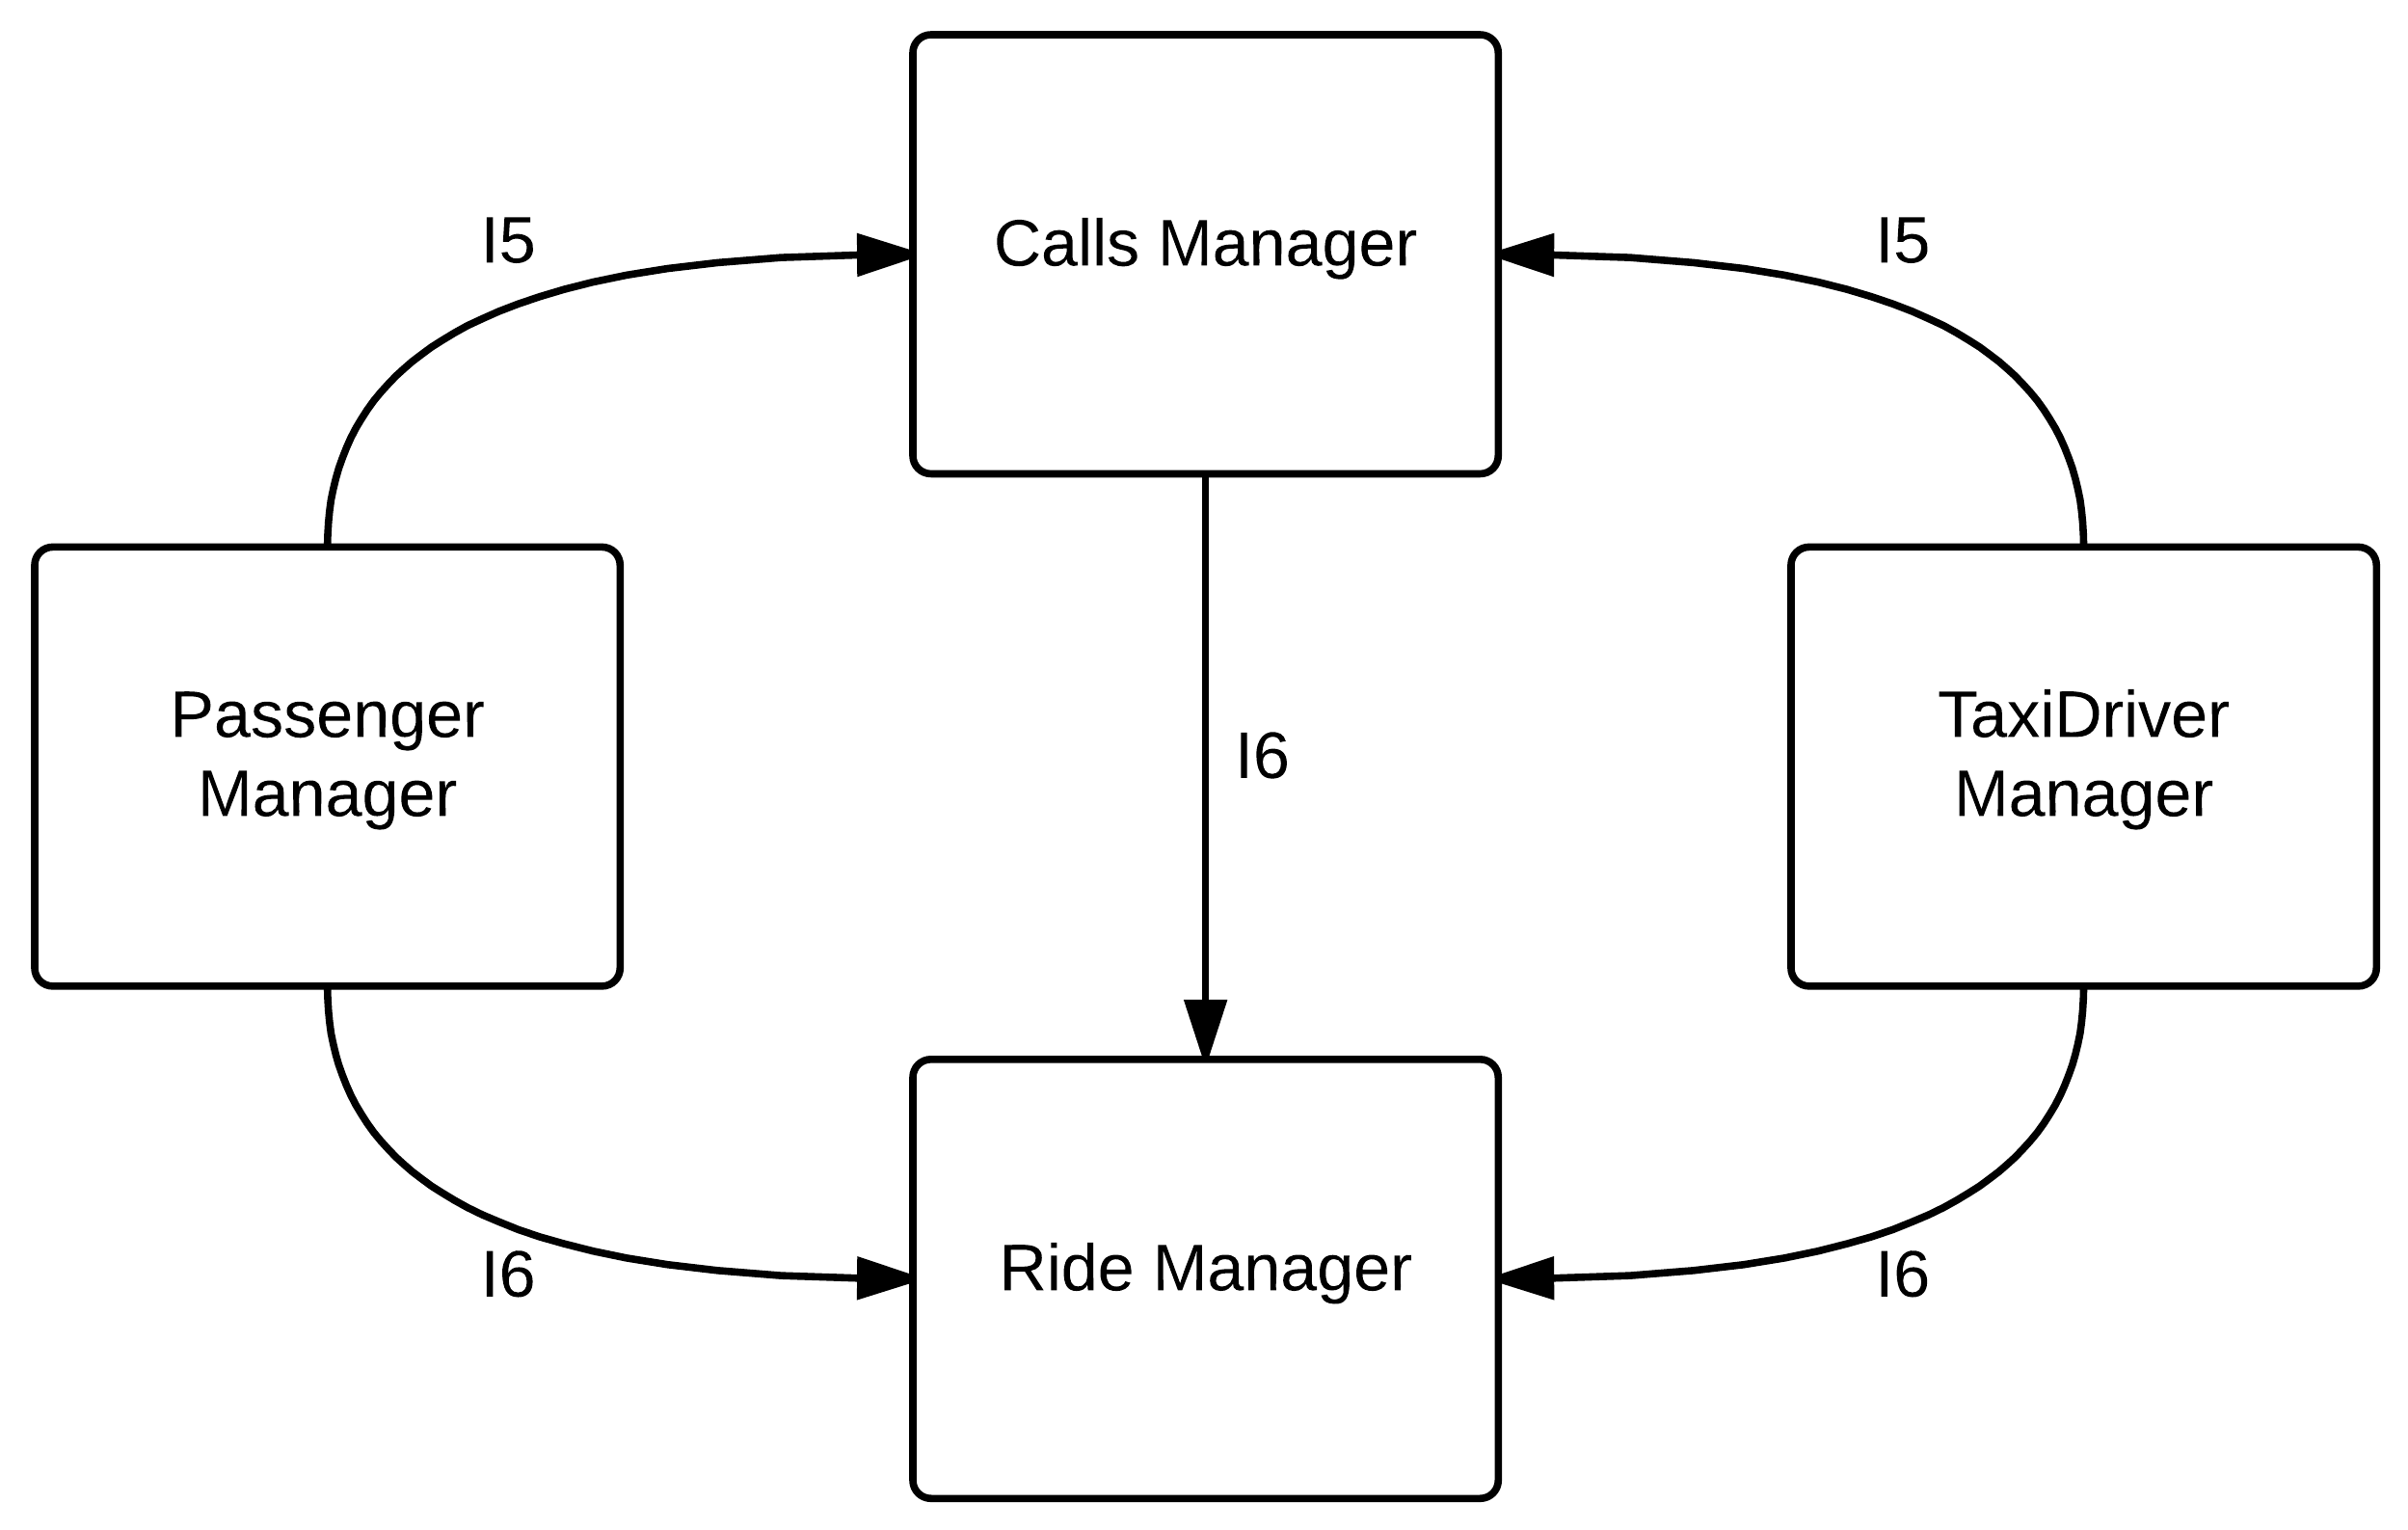
\includegraphics[width=\textwidth]{cpt/img/ITDPComponentDiagramsTP2}
\end{figure}

\begin{table}[!htbp]
\begin{center}
\begin{tabular}[t]{c|p{0.7\textwidth}|c}

\textbf{ID} & \textbf{Integration Test} & \textbf{Paragraphs} \\
\hline
I5 & Passenger Manager, TaxiDriver Manager $\rightarrow$ Calls Manager & 3.1.5  3.2.2\\
\hline
I6 & Passenger Manager, TaxiDriver Manager, Calls Manager $\rightarrow$ Ride Manager & 3.1.6  3.2.2\\
\hline
\end{tabular}
\end{center}
\end{table}
\clearpage

\begin{figure}[!htbp]
\centering
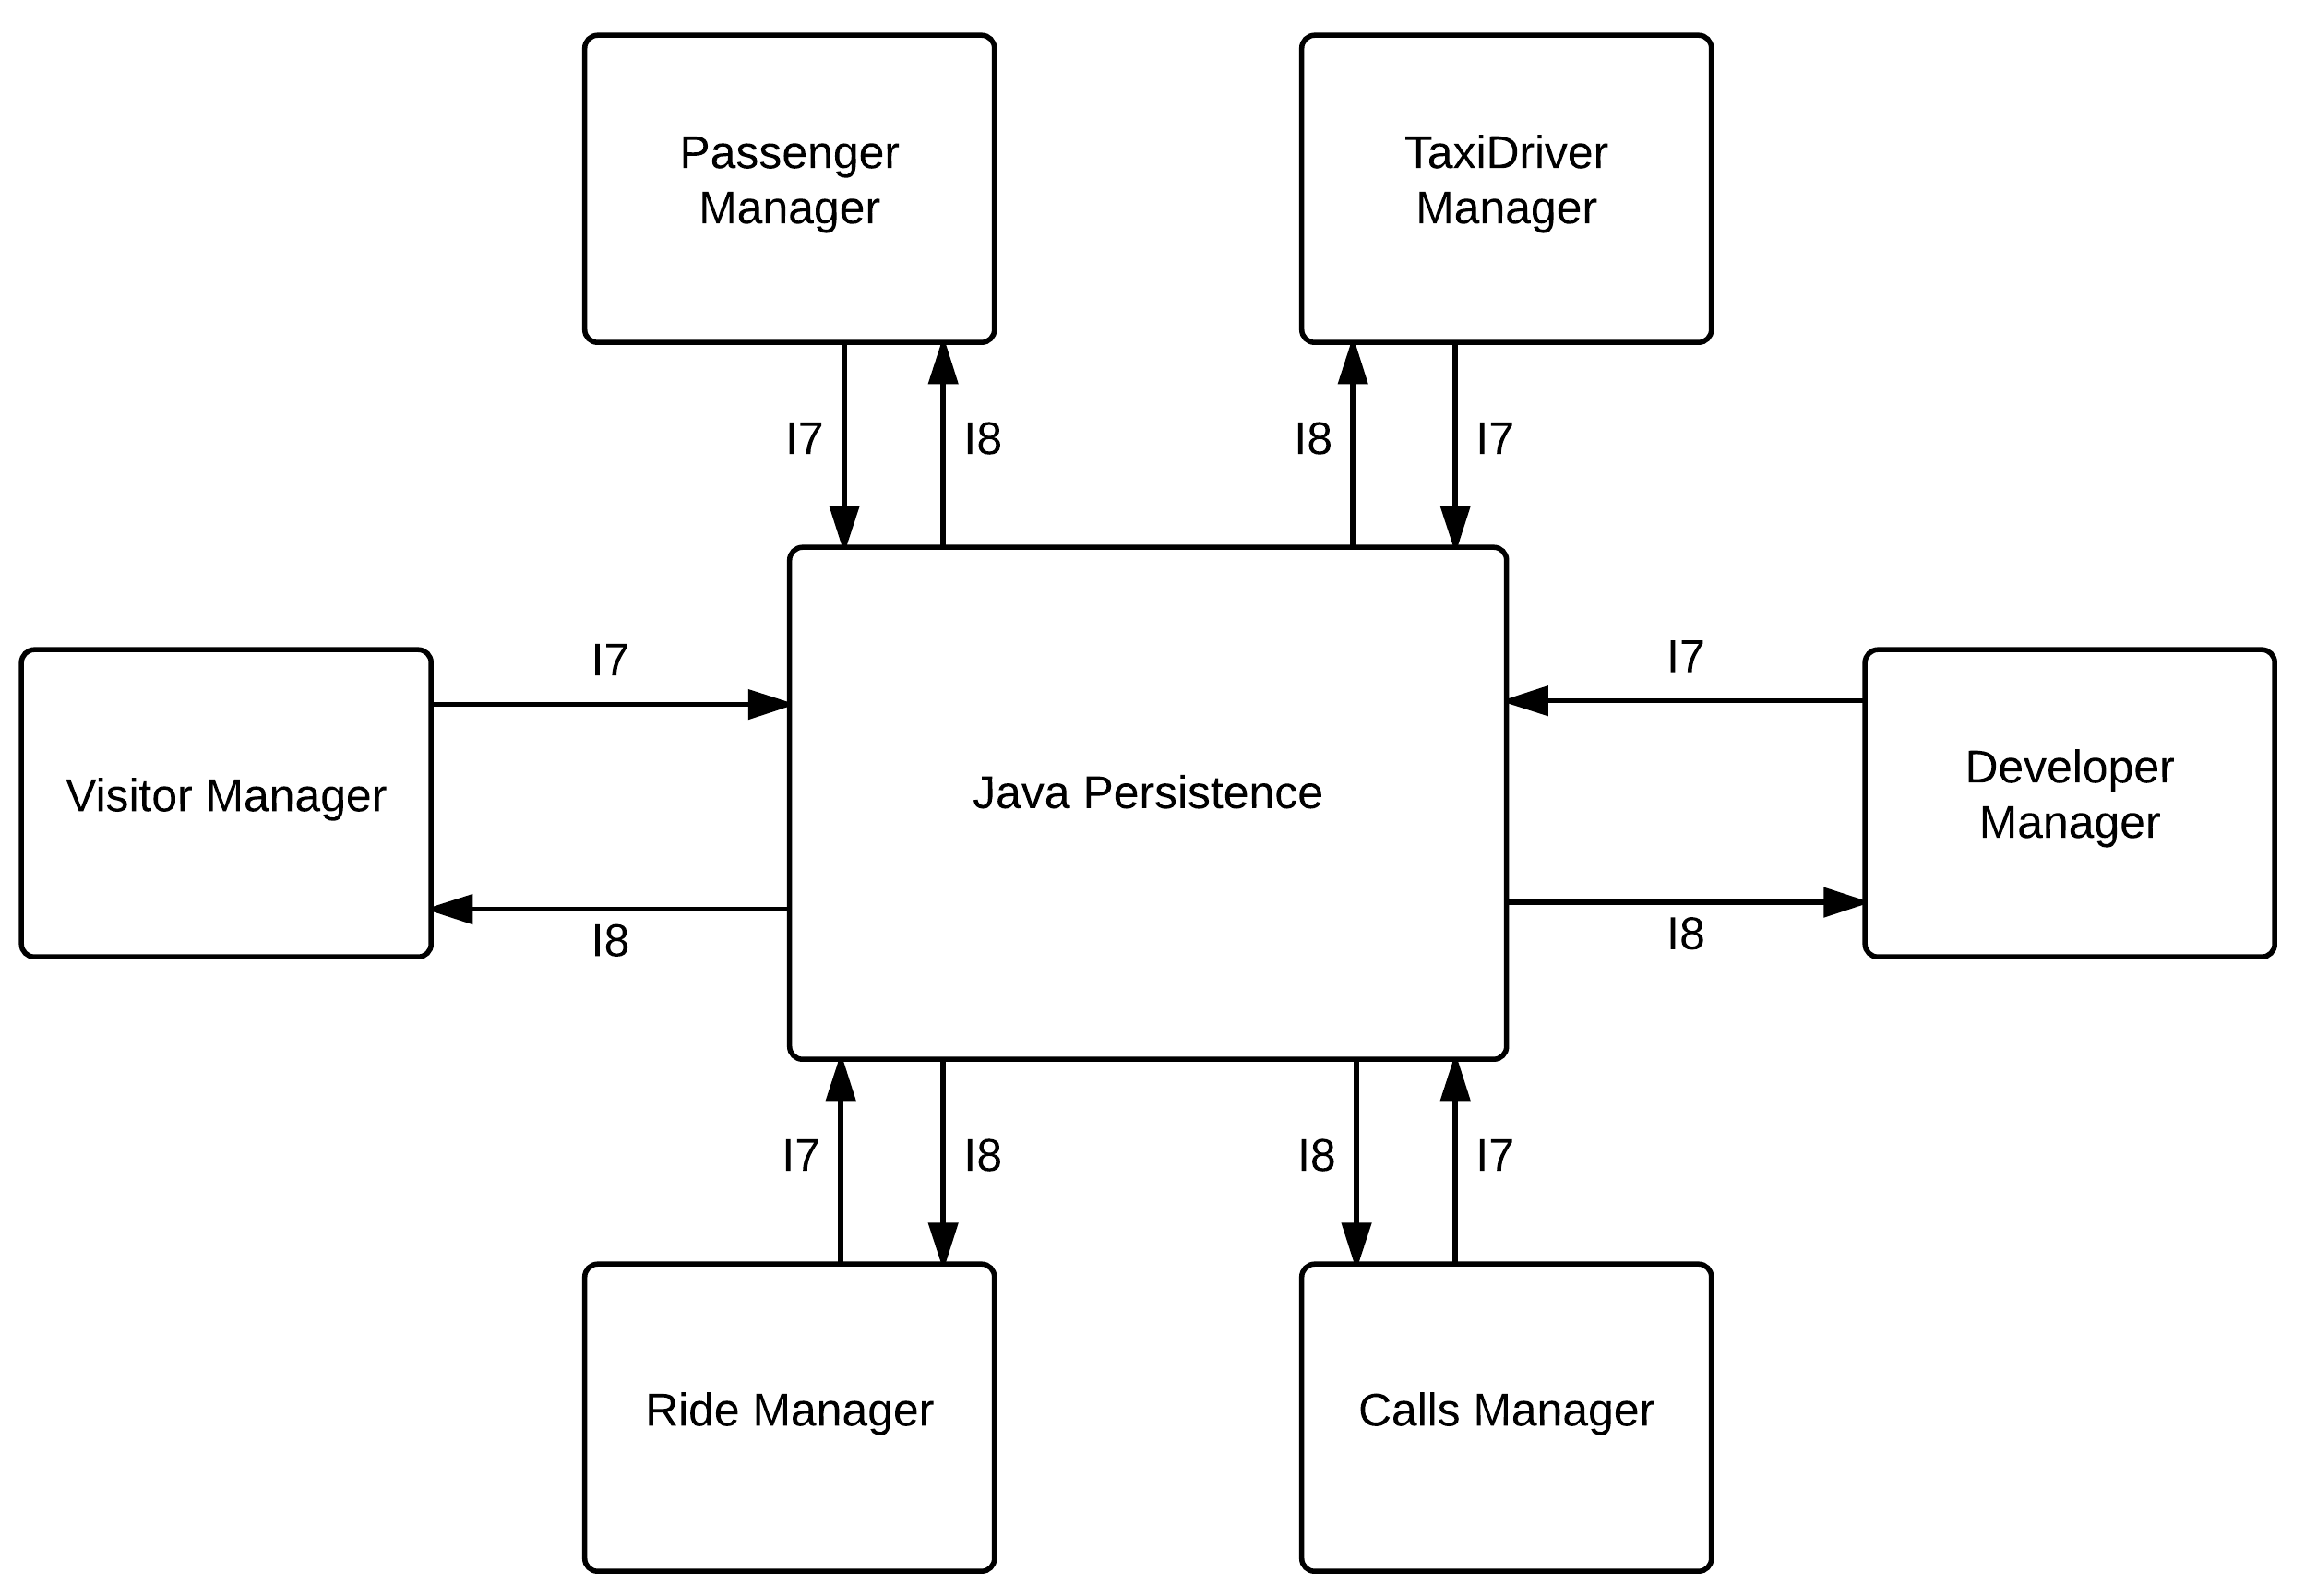
\includegraphics[width=\textwidth]{cpt/img/ITDPComponentDiagramsTP3}
\end{figure}

\begin{table}[!htbp]
\begin{center}
\begin{tabular}[t]{c|p{0.7\textwidth}|c}

\textbf{ID} & \textbf{Integration Test} & \textbf{Paragraphs} \\
\hline
I7 & Visitor Manager, Passenger Manager, TaxiDriver Manager, Developer Manager, Calls Manager, Ride Manager $\rightarrow$ Java Persistence & 3.1.7  3.2.3 \\
\hline
I8 & Java Persistence $\rightarrow$ Visitor Manager, Passenger Manager, TaxiDriver Manager, Developer Manager, Calls Manager, Ride Manager & 3.1.8  3.2.3 \\
\hline
\end{tabular}
\end{center}
\end{table}
\clearpage

\begin{figure}[!htbp]
\centering
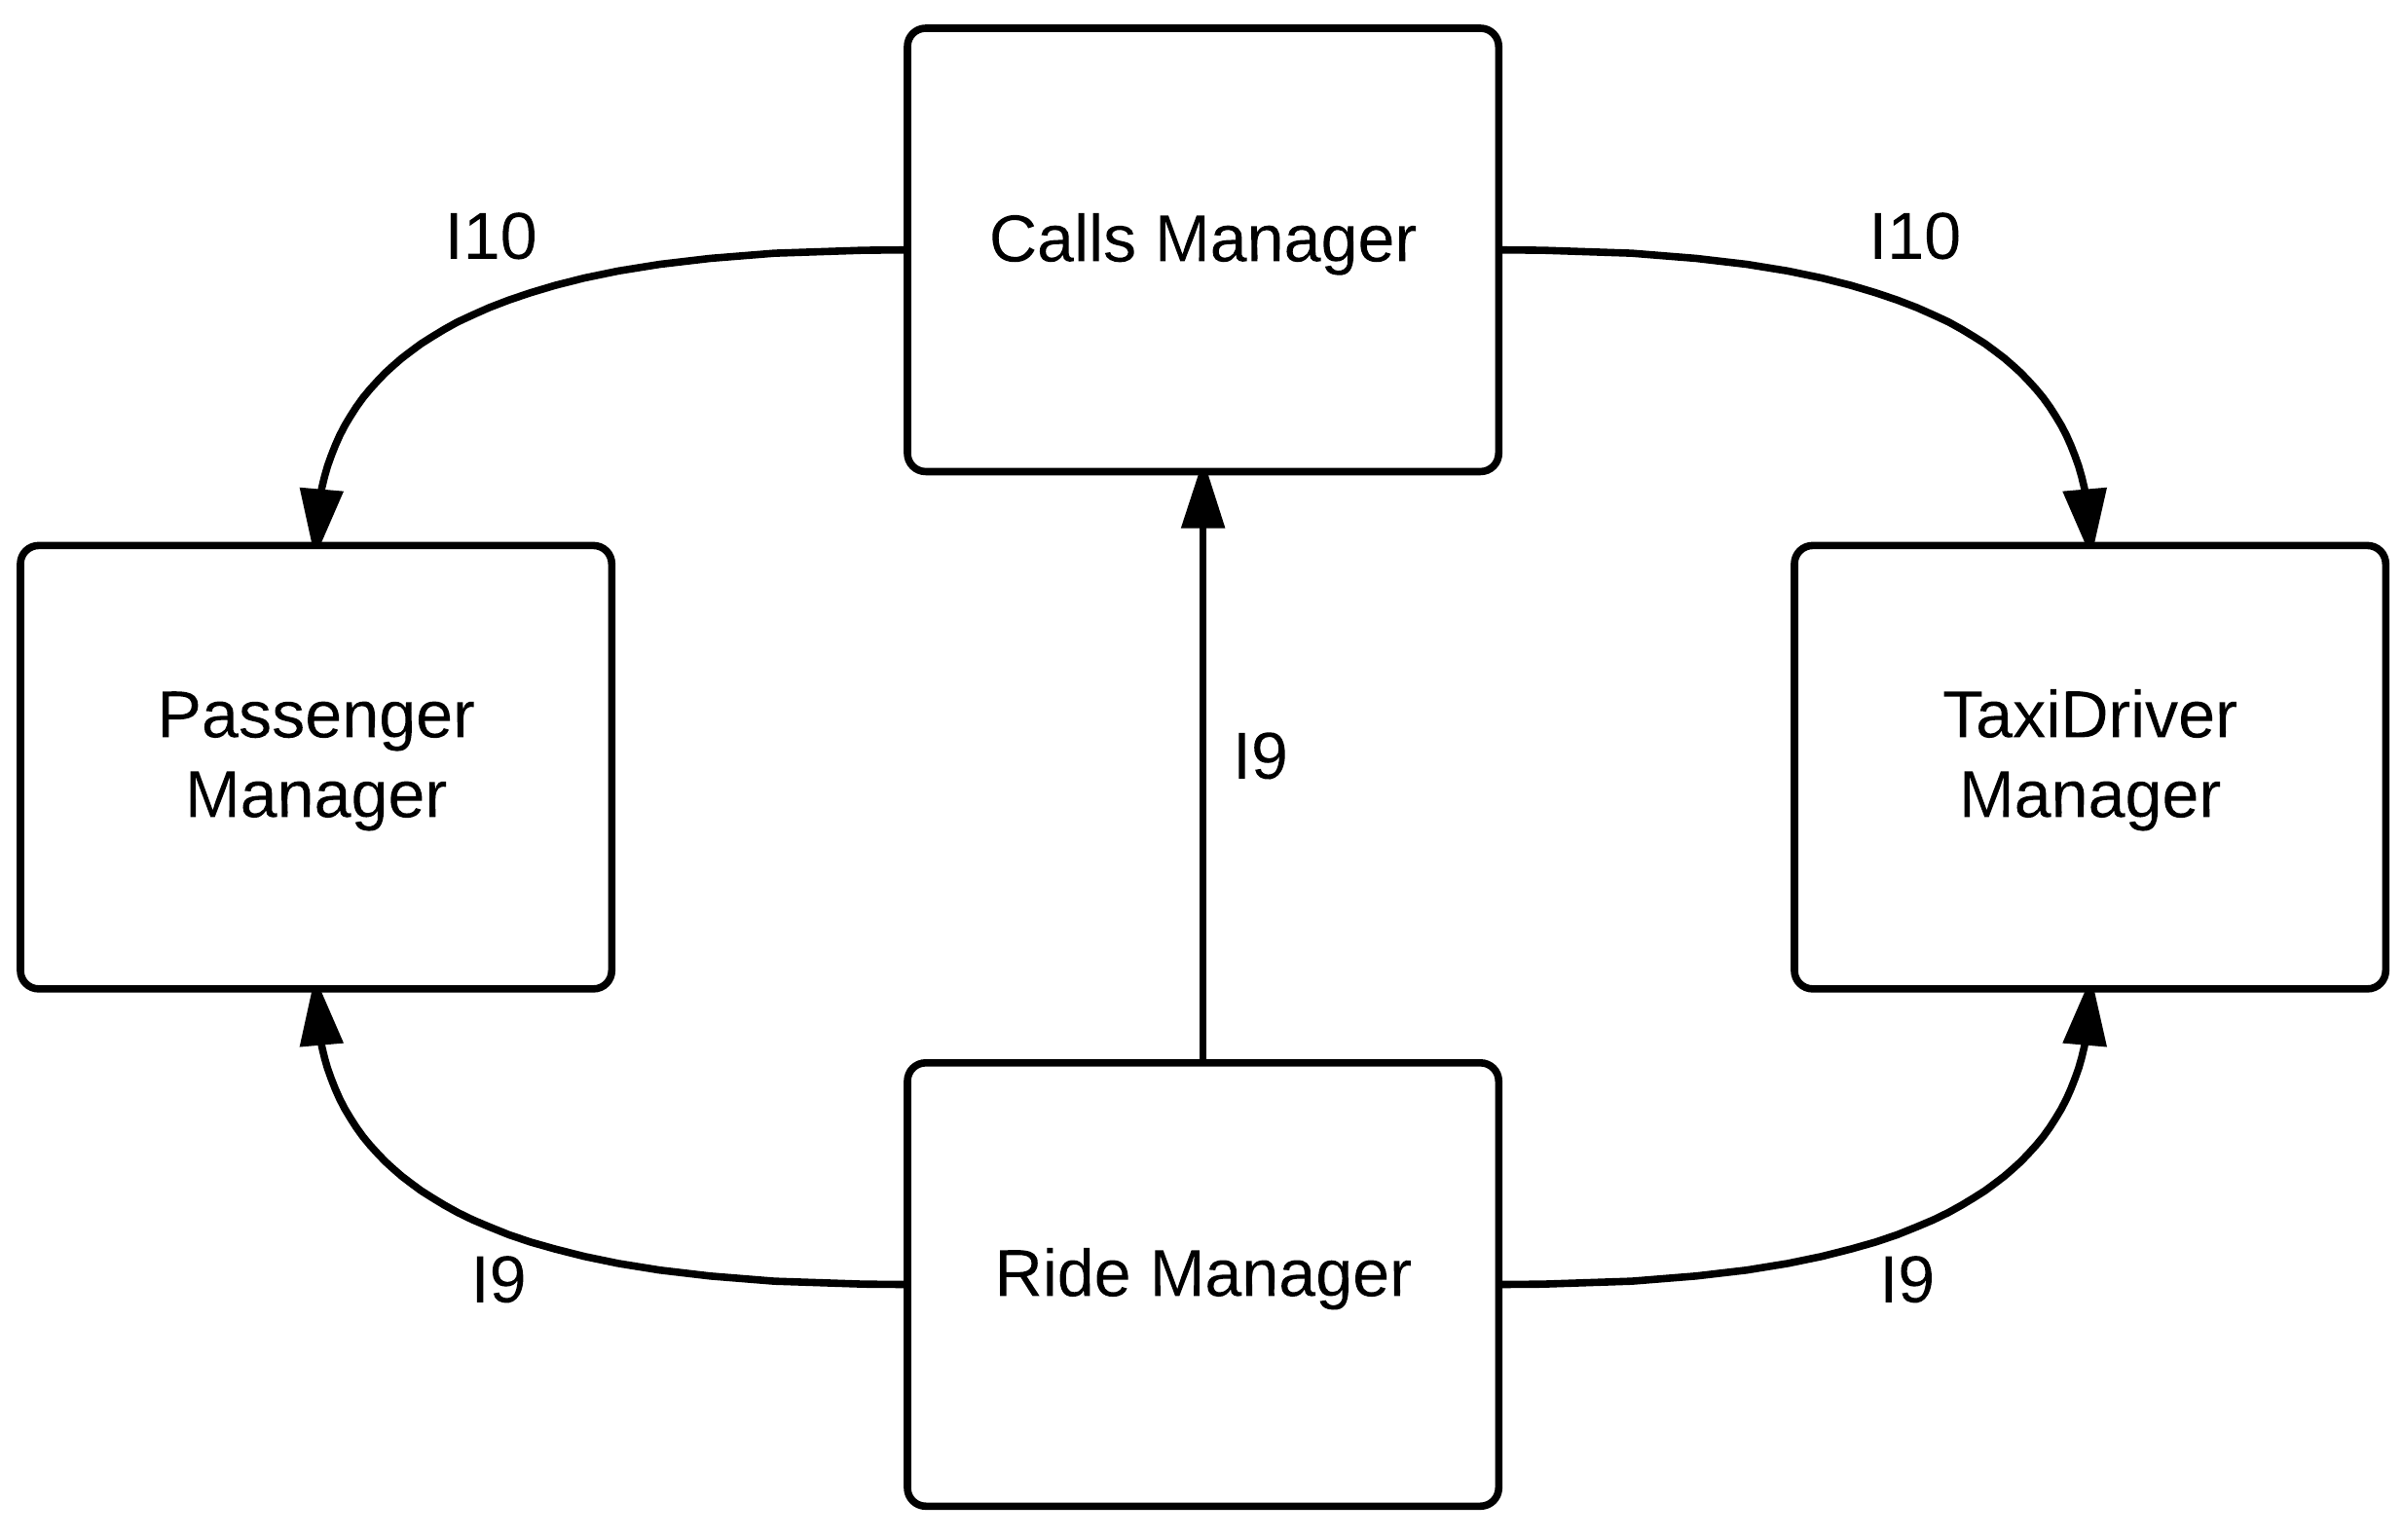
\includegraphics[width=\textwidth]{cpt/img/ITDPComponentDiagramsTP4}
\end{figure}

\begin{table}[!htbp]
\begin{center}
\begin{tabular}[t]{c|p{0.7\textwidth}|c}

\textbf{ID} & \textbf{Integration Test} & \textbf{Paragraphs} \\
\hline
I9 &  Ride Manager $\rightarrow$ Passenger Manager, TaxiDriver Manager, Calls Manager & 3.1.9  3.2.4\\
\hline
I10 & Calls Manager $\rightarrow$ Passenger Manager, TaxiDriver Manager & 3.1.10  3.2.4\\
\hline
\end{tabular}
\end{center}
\end{table}
\clearpage

\begin{figure}[!htbp]
\centering
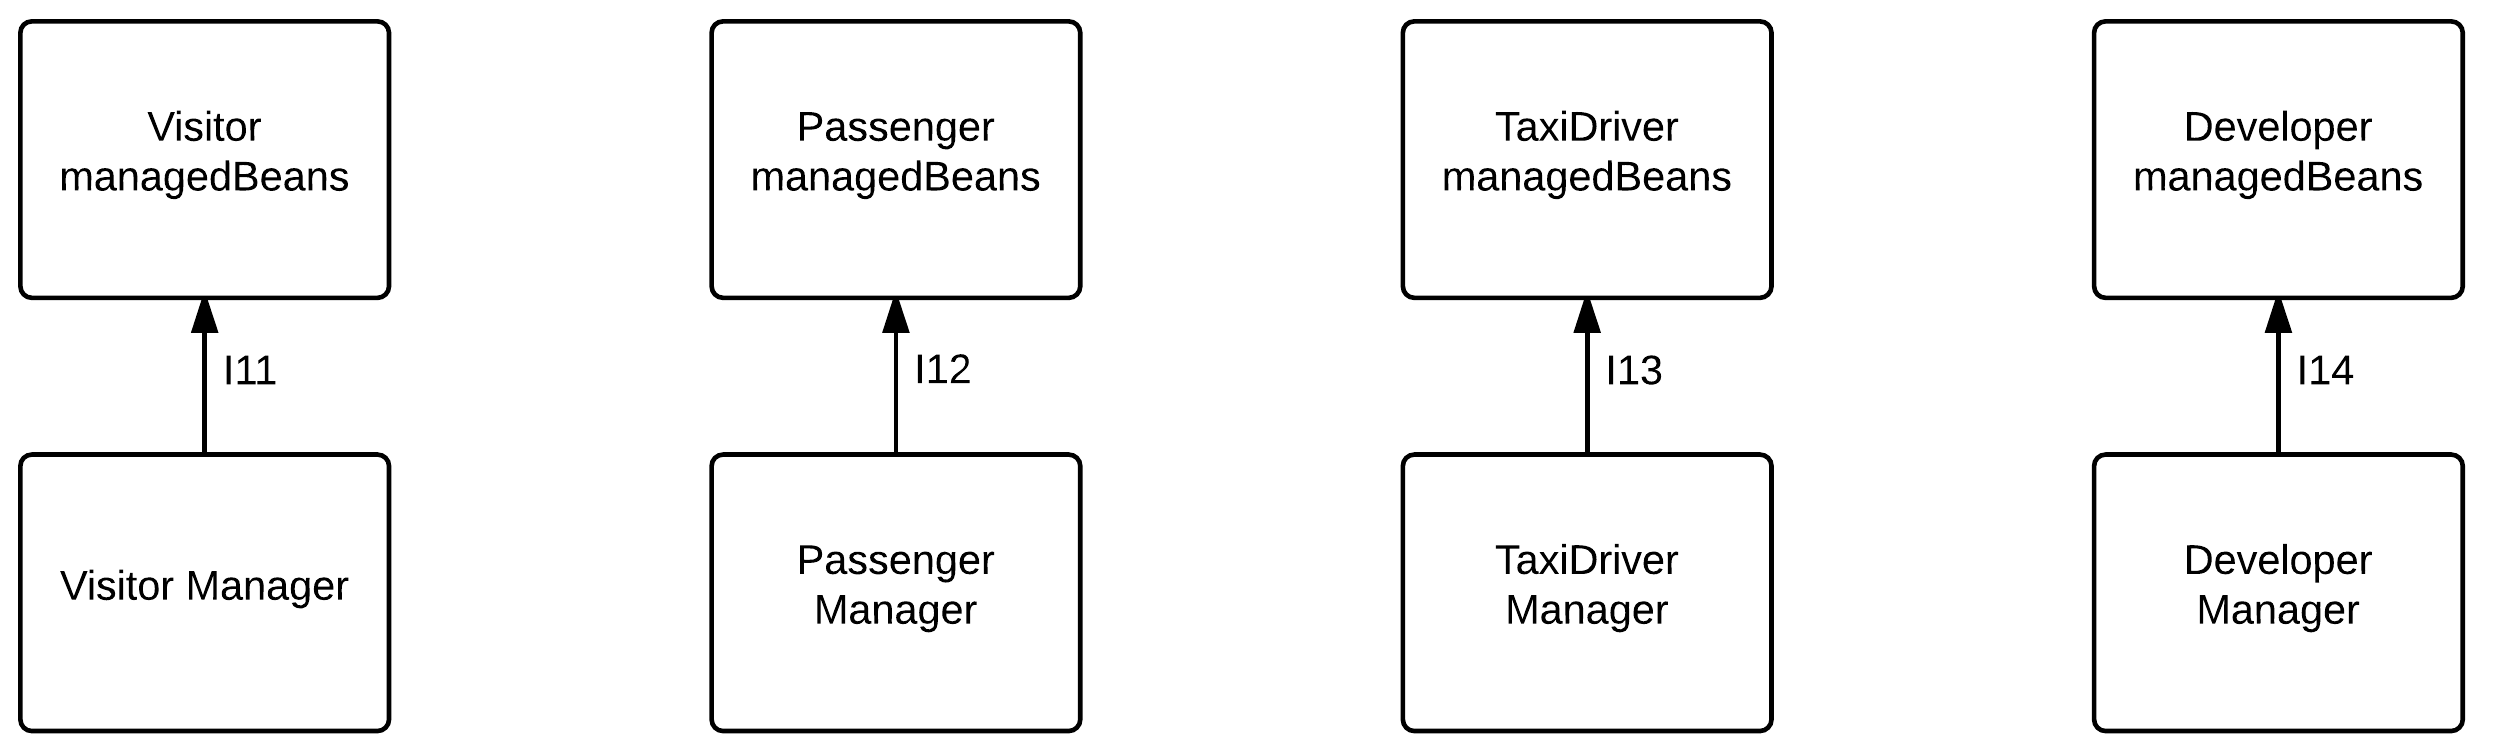
\includegraphics[width=\textwidth]{cpt/img/ITDPComponentDiagramsTP5}
\end{figure}

\begin{table}[!htbp]
\begin{center}
\begin{tabular}[t]{c|p{0.7\textwidth}|c}

\textbf{ID} & \textbf{Integration Test} & \textbf{Paragraphs} \\
\hline
I11 & Visitor Manager $\rightarrow$ Visitor managedBean & 3.1.11  3.2.5 \\
\hline
I12 & Passenger Manager $\rightarrow$ Passenger managedBean & 3.1.12  3.2.5 \\
\hline
I13 & TaxiDriver Manager $\rightarrow$ TaxiDriver managedBean & 3.1.13  3.2.5 \\
\hline
I14 & Developer Manager $\rightarrow$ Developer managedBean & 3.1.14  3.2.5 \\
\hline

\end{tabular}
\end{center}
\end{table}
\clearpage
\clearpage

\chapter{Individual Steps \& Test Description} \label{chap3}

\section{Test case specifications}


\subsection{Integration test case I1}

\begin{table}[!htbp]
\begin{center}
\begin{tabular}[t]{p{0.35\textwidth}|p{0.65\textwidth}}

\hline
\textbf{Test Case Identifier} & I1T1 \\
\hline
\textbf{Test Item} & Visitor managedBeans $\rightarrow$ Visitor Manager \\
\hline
\textbf{Input Specification} & Create typical Visitor managedBeans input  \\
\hline
\textbf{Output Specification} & Check if the correct methods are called in the Visitor Manager \\
\hline
\textbf{Environmental Needs} & Client driver \\
\hline

\end{tabular}
\end{center}
\end{table}
\clearpage

\subsection{Integration test case I2}

\begin{table}[!htbp]
\begin{center}
\begin{tabular}[t]{p{0.35\textwidth}|p{0.65\textwidth}}

\hline
\textbf{Test Case Identifier} & I2T1 \\
\hline
\textbf{Test Item} & Passenger managedBeans $\rightarrow$ Passenger Manager \\
\hline
\textbf{Input Specification} & Create typical Passenger managedBeans input  \\
\hline
\textbf{Output Specification} & Check if the correct methods are called in the Passenger Manager \\
\hline
\textbf{Environmental Needs} & Client driver \\
\hline

\end{tabular}
\end{center}
\end{table}

\subsection{Integration test case I3}

\begin{table}[!htbp]
\begin{center}
\begin{tabular}[t]{p{0.35\textwidth}|p{0.65\textwidth}}

\hline
\textbf{Test Case Identifier} & I3T1 \\
\hline
\textbf{Test Item} & TaxiDriver managedBeans $\rightarrow$ TaxiDriver Manager \\
\hline
\textbf{Input Specification} & Create typical TaxiDriver managedBeans input  \\
\hline
\textbf{Output Specification} & Check if the correct methods are called in the TaxiDriver Manager \\
\hline
\textbf{Environmental Needs} & Client driver \\
\hline

\end{tabular}
\end{center}
\end{table}

\subsection{Integration test case I4}

\begin{table}[!htbp]
\begin{center}
\begin{tabular}[t]{p{0.35\textwidth}|p{0.65\textwidth}}

\hline
\textbf{Test Case Identifier} & I4T1 \\
\hline
\textbf{Test Item} & Developer managedBeans $\rightarrow$ Developer Manager \\
\hline
\textbf{Input Specification} & Create typical Developer managedBeans input  \\
\hline
\textbf{Output Specification} & Check if the correct methods are called in the Developer Manager \\
\hline
\textbf{Environmental Needs} & Client driver \\
\hline

\end{tabular}
\end{center}
\end{table}
\clearpage


\subsection{Integration test case I5}

\begin{table}[!htbp]
\begin{center}
\begin{tabular}[t]{p{0.35\textwidth}|p{0.65\textwidth}}

\hline
\textbf{Test Case Identifier} & I5T1 \\
\hline
\textbf{Test Item} & Passenger Manager $\rightarrow$ Calls Manager \\
\hline
\textbf{Input Specification} & Create typical Passenger Manager input \\
\hline
\textbf{Output Specification} & Check if the correct methods are called in the Calls Manager \\
\hline
\textbf{Environmental Needs} & I2 succeded \\
\hline

\end{tabular}
\end{center}
\end{table}

\begin{table}[!htbp]
\begin{center}
\begin{tabular}[t]{p{0.35\textwidth}|p{0.65\textwidth}}

\hline
\textbf{Test Case Identifier} & I5T2 \\
\hline
\textbf{Test Item} & TaxiDriver Manager $\rightarrow$ Calls Manager \\
\hline
\textbf{Input Specification} & Create typical TaxiDriver Manager input \\
\hline
\textbf{Output Specification} & Check if the correct methods are called in the Calls Manager \\
\hline
\textbf{Environmental Needs} & I3 succeded \\
\hline

\end{tabular}
\end{center}
\end{table}

\subsection{Integration test case I6}

\begin{table}[!htbp]
\begin{center}
\begin{tabular}[t]{p{0.35\textwidth}|p{0.65\textwidth}}

\hline
\textbf{Test Case Identifier} & I6T1 \\
\hline
\textbf{Test Item} & Passenger Manager $\rightarrow$ Ride Manager \\
\hline
\textbf{Input Specification} & Create typical Passenger Manager input \\
\hline
\textbf{Output Specification} & Check if the correct methods are called in the Ride Manager \\
\hline
\textbf{Environmental Needs} & I2 succeded \\
\hline

\end{tabular}
\end{center}
\end{table}

\begin{table}[!htbp]
\begin{center}
\begin{tabular}[t]{p{0.35\textwidth}|p{0.65\textwidth}}

\hline
\textbf{Test Case Identifier} & I6T2 \\
\hline
\textbf{Test Item} & TaxiDriver Manager $\rightarrow$ Ride Manager \\
\hline
\textbf{Input Specification} & Create typical TaxiDriver Manager input \\
\hline
\textbf{Output Specification} & Check if the correct methods are called in the Ride Manager \\
\hline
\textbf{Environmental Needs} & I3 succeded \\
\hline

\end{tabular}
\end{center}
\end{table}

\begin{table}[!htbp]
\begin{center}
\begin{tabular}[t]{p{0.35\textwidth}|p{0.65\textwidth}}

\hline
\textbf{Test Case Identifier} & I6T3 \\
\hline
\textbf{Test Item} & Calls Manager $\rightarrow$ Ride Manager \\
\hline
\textbf{Input Specification} & Create typical Calls Manager input \\
\hline
\textbf{Output Specification} & Check if the correct methods are called in the Ride Manager \\
\hline
\textbf{Environmental Needs} & I2, I3, I5 succeded \\
\hline

\end{tabular}
\end{center}
\end{table}
\clearpage

\subsection{Integration test case I7}

\begin{table}[!htbp]
\begin{center}
\begin{tabular}[t]{p{0.35\textwidth}|p{0.65\textwidth}}

\hline
\textbf{Test Case Identifier} & I7T1 \\
\hline
\textbf{Test Item} & Visitor Manager $\rightarrow$ Java Persistence \\
\hline
\textbf{Input Specification} & Create typical Visitor Manager input  \\
\hline
\textbf{Output Specification} & Check if the correct methods are called in the Persistence Module \\
\hline
\textbf{Environmental Needs} & I1 succeded \\
\hline

\end{tabular}
\end{center}
\end{table}

\begin{table}[!htbp]
\begin{center}
\begin{tabular}[t]{p{0.35\textwidth}|p{0.65\textwidth}}

\hline
\textbf{Test Case Identifier} & I7T2 \\
\hline
\textbf{Test Item} & Passenger Manager $\rightarrow$ Java Persistence \\
\hline
\textbf{Input Specification} & Create typical Passenger Manager input \\
\hline
\textbf{Output Specification} & Check if the correct methods are called in the Persistence Module \\
\hline
\textbf{Environmental Needs} & I2 succeded \\
\hline

\end{tabular}
\end{center}
\end{table}

\begin{table}[!htbp]
\begin{center}
\begin{tabular}[t]{p{0.35\textwidth}|p{0.65\textwidth}}

\hline
\textbf{Test Case Identifier} & I7T3 \\
\hline
\textbf{Test Item} & TaxiDriver Manager $\rightarrow$ Java Persistence \\
\hline
\textbf{Input Specification} & Create typical TaxiDriver Manager input \\
\hline
\textbf{Output Specification} & Check if the correct methods are called in the Persistence Module \\
\hline
\textbf{Environmental Needs} & I3 succeded \\
\hline

\end{tabular}
\end{center}
\end{table}

\begin{table}[!htbp]
\begin{center}
\begin{tabular}[t]{p{0.35\textwidth}|p{0.65\textwidth}}

\hline
\textbf{Test Case Identifier} & I7T4 \\
\hline
\textbf{Test Item} & Developer Manager $\rightarrow$ Java Persistence \\
\hline
\textbf{Input Specification} & Create typical Developer Manager input \\
\hline
\textbf{Output Specification} & Check if the correct methods are called in the Persistence Module \\
\hline
\textbf{Environmental Needs} & I4 succeded \\
\hline

\end{tabular}
\end{center}
\end{table}

\begin{table}[!htbp]
\begin{center}
\begin{tabular}[t]{p{0.35\textwidth}|p{0.65\textwidth}}

\hline
\textbf{Test Case Identifier} & I7T5 \\
\hline
\textbf{Test Item} & Calls Manager $\rightarrow$ Java Persistence \\
\hline
\textbf{Input Specification} & Create typical Calls Manager input \\
\hline
\textbf{Output Specification} & Check if the correct methods are called in the Persistence Module \\
\hline
\textbf{Environmental Needs} & I2, I3 and I5 succeded \\
\hline

\end{tabular}
\end{center}
\end{table}

\begin{table}[!htbp]
\begin{center}
\begin{tabular}[t]{p{0.35\textwidth}|p{0.65\textwidth}}

\hline
\textbf{Test Case Identifier} & I7T6 \\
\hline
\textbf{Test Item} & Ride Manager $\rightarrow$ Java Persistence \\
\hline
\textbf{Input Specification} & Create typical Ride Manager input \\
\hline
\textbf{Output Specification} & Check if the correct methods are called in the Persistence Module \\
\hline
\textbf{Environmental Needs} & I2, I3, I5 and I6 succeded \\
\hline

\end{tabular}
\end{center}
\end{table}
\clearpage

\subsection{Integration test case I8}

\begin{table}[!htbp]
\begin{center}
\begin{tabular}[t]{p{0.35\textwidth}|p{0.65\textwidth}}

\hline
\textbf{Test Case Identifier} & I8T1 \\
\hline
\textbf{Test Item} & Java Persistence $\rightarrow$ Visitor Manager \\
\hline
\textbf{Input Specification} & Create typical Java Persistence input  \\
\hline
\textbf{Output Specification} & Check if the correct methods are called in the Visitor Manager \\
\hline
\textbf{Environmental Needs} & Database Driver \\
\hline

\end{tabular}
\end{center}
\end{table}

\begin{table}[!htbp]
\begin{center}
\begin{tabular}[t]{p{0.35\textwidth}|p{0.65\textwidth}}

\hline
\textbf{Test Case Identifier} & I8T2 \\
\hline
\textbf{Test Item} & Java Persistence $\rightarrow$ Passenger Manager \\
\hline
\textbf{Input Specification} & Create typical Java Persistence input \\
\hline
\textbf{Output Specification} & Check if the correct methods are called in the Passenger Manager \\
\hline
\textbf{Environmental Needs} & Database Driver \\
\hline

\end{tabular}
\end{center}
\end{table}

\begin{table}[!htbp]
\begin{center}
\begin{tabular}[t]{p{0.35\textwidth}|p{0.65\textwidth}}

\hline
\textbf{Test Case Identifier} & I8T3 \\
\hline
\textbf{Test Item} & Java Persistence $\rightarrow$ TaxiDriver Manager \\
\hline
\textbf{Input Specification} & Create typical Java Persistence input \\
\hline
\textbf{Output Specification} & Check if the correct methods are called in the TaxiDriver Manager \\
\hline
\textbf{Environmental Needs} & Database Driver \\
\hline

\end{tabular}
\end{center}
\end{table}

\begin{table}[!htbp]
\begin{center}
\begin{tabular}[t]{p{0.35\textwidth}|p{0.65\textwidth}}

\hline
\textbf{Test Case Identifier} & I8T4 \\
\hline
\textbf{Test Item} & Java Persistence $\rightarrow$ Developer Manager \\
\hline
\textbf{Input Specification} & Create typical Java Persistence input \\
\hline
\textbf{Output Specification} & Check if the correct methods are called in the Developer Manager \\
\hline
\textbf{Environmental Needs} & Database Driver \\
\hline

\end{tabular}
\end{center}
\end{table}

\begin{table}[!htbp]
\begin{center}
\begin{tabular}[t]{p{0.35\textwidth}|p{0.65\textwidth}}

\hline
\textbf{Test Case Identifier} & I8T5 \\
\hline
\textbf{Test Item} & Java Persistence $\rightarrow$ Calls Manager \\
\hline
\textbf{Input Specification} & Create typical Java Persistence input \\
\hline
\textbf{Output Specification} & Check if the correct methods are called in the Calls Manager \\
\hline
\textbf{Environmental Needs} & Database Driver \\
\hline

\end{tabular}
\end{center}
\end{table}

\begin{table}[!htbp]
\begin{center}
\begin{tabular}[t]{p{0.35\textwidth}|p{0.65\textwidth}}

\hline
\textbf{Test Case Identifier} & I8T6 \\
\hline
\textbf{Test Item} & Java Persistence $\rightarrow$ Ride Manager \\
\hline
\textbf{Input Specification} & Create typical Java Persistence input \\
\hline
\textbf{Output Specification} & Check if the correct methods are called in the Ride Manager \\
\hline
\textbf{Environmental Needs} & Database Driver \\
\hline

\end{tabular}
\end{center}
\end{table}
\clearpage


\subsection{Integration test case I9}

\begin{table}[!htbp]
\begin{center}
\begin{tabular}[t]{p{0.35\textwidth}|p{0.65\textwidth}}

\hline
\textbf{Test Case Identifier} & I9T1 \\
\hline
\textbf{Test Item} & Ride Manager $\rightarrow$ Passenger Manager \\
\hline
\textbf{Input Specification} & Create typical Ride Manager input \\
\hline
\textbf{Output Specification} & Check if the correct methods are called in the Passenger Manager \\
\hline
\textbf{Environmental Needs} & I8 succeded \\
\hline

\end{tabular}
\end{center}
\end{table}

\begin{table}[!htbp]
\begin{center}
\begin{tabular}[t]{p{0.35\textwidth}|p{0.65\textwidth}}

\hline
\textbf{Test Case Identifier} & I9T2 \\
\hline
\textbf{Test Item} & Ride Manager $\rightarrow$ TaxiDriver Manager \\
\hline
\textbf{Input Specification} & Create typical Ride Manager input \\
\hline
\textbf{Output Specification} & Check if the correct methods are called in the TaxiDriver Manager \\
\hline
\textbf{Environmental Needs} & I8 succeded \\
\hline

\end{tabular}
\end{center}
\end{table}

\begin{table}[!htbp]
\begin{center}
\begin{tabular}[t]{p{0.35\textwidth}|p{0.65\textwidth}}

\hline
\textbf{Test Case Identifier} & I9T3 \\
\hline
\textbf{Test Item} & Ride Manager $\rightarrow$ Calls Manager \\
\hline
\textbf{Input Specification} & Create typical Ride Manager input \\
\hline
\textbf{Output Specification} & Check if the correct methods are called in the Calls Manager \\
\hline
\textbf{Environmental Needs} & I8 succeded \\
\hline

\end{tabular}
\end{center}
\end{table}
\clearpage


\subsection{Integration test case I10}

\begin{table}[!htbp]
\begin{center}
\begin{tabular}[t]{p{0.35\textwidth}|p{0.65\textwidth}}

\hline
\textbf{Test Case Identifier} & I10T1 \\
\hline
\textbf{Test Item} & Calls Manager $\rightarrow$ Passenger Manager \\
\hline
\textbf{Input Specification} & Create typical Calls Manager input \\
\hline
\textbf{Output Specification} & Check if the correct methods are called in the Passenger Manager \\
\hline
\textbf{Environmental Needs} & I8 and I9 succeded \\
\hline

\end{tabular}
\end{center}
\end{table}

\begin{table}[!htbp]
\begin{center}
\begin{tabular}[t]{p{0.35\textwidth}|p{0.65\textwidth}}

\hline
\textbf{Test Case Identifier} & I10T2 \\
\hline
\textbf{Test Item} & Calls Manager $\rightarrow$ TaxiDriver Manager \\
\hline
\textbf{Input Specification} & Create typical Calls Manager input \\
\hline
\textbf{Output Specification} & Check if the correct methods are called in the TaxiDriver Manager \\
\hline
\textbf{Environmental Needs} & I8 and I9 succeded \\
\hline

\end{tabular}
\end{center}
\end{table}

\subsection{Integration test case I11}

\begin{table}[!htbp]
\begin{center}
\begin{tabular}[t]{p{0.35\textwidth}|p{0.65\textwidth}}

\hline
\textbf{Test Case Identifier} & I11T1 \\
\hline
\textbf{Test Item} & Visitor Manager $\rightarrow$ Visitor managedBeans \\
\hline
\textbf{Input Specification} & Create typical Visitor Manager input  \\
\hline
\textbf{Output Specification} & Check if the correct methods are called in the Visitor managedBeans \\
\hline
\textbf{Environmental Needs} & I8 succeded \\
\hline

\end{tabular}
\end{center}
\end{table}
\clearpage


\subsection{Integration test case I12}

\begin{table}[!htbp]
\begin{center}
\begin{tabular}[t]{p{0.35\textwidth}|p{0.65\textwidth}}

\hline
\textbf{Test Case Identifier} & I12T1 \\
\hline
\textbf{Test Item} & Passenger Manager $\rightarrow$ Passenger managedBeans \\
\hline
\textbf{Input Specification} & Create typical Passenger Manager input  \\
\hline
\textbf{Output Specification} & Check if the correct methods are called in the Passenger managedBeans \\
\hline
\textbf{Environmental Needs} & I8, I9 and I10 succeded \\
\hline

\end{tabular}
\end{center}
\end{table}

\subsection{Integration test case I13}

\begin{table}[!htbp]
\begin{center}
\begin{tabular}[t]{p{0.35\textwidth}|p{0.65\textwidth}}

\hline
\textbf{Test Case Identifier} & I13T1 \\
\hline
\textbf{Test Item} & TaxiDriver Manager $\rightarrow$ TaxiDriver managedBeans \\
\hline
\textbf{Input Specification} & Create typical TaxiDriver Manager input  \\
\hline
\textbf{Output Specification} & Check if the correct methods are called in the TaxiDriver managedBeans \\
\hline
\textbf{Environmental Needs} & I8, I9 and I10 succeded \\
\hline

\end{tabular}
\end{center}
\end{table}

\subsection{Integration test case I14}

\begin{table}[!htbp]
\begin{center}
\begin{tabular}[t]{p{0.35\textwidth}|p{0.65\textwidth}}

\hline
\textbf{Test Case Identifier} & I14T1 \\
\hline
\textbf{Test Item} & Developer Manager $\rightarrow$ Developer managedBeans \\
\hline
\textbf{Input Specification} & Create typical Developer Manager input  \\
\hline
\textbf{Output Specification} & Check if the correct methods are called in the Developer managedBeans \\
\hline
\textbf{Environmental Needs} & I8 succeded \\
\hline

\end{tabular}
\end{center}
\end{table}
\clearpage

\section{Test procedures}

\subsection{Test procedure TP1}

\begin{table}[!htbp]
\begin{center}
\begin{tabular}[t]{p{0.35\textwidth}|p{0.65\textwidth}}

\hline
\textbf{Test Procedure Identifier} & TP1 \\
\hline
\textbf{Purpose} & This test procedure verifies whether all the Managers of the Business Layer can successfully:
\begin{itemize*}
	\item receive requests from the corresponding managedBeans
	\item correctly elaborate those requests
\end{itemize*} \\
\hline
\textbf{Procedure Steps} & Execute I1, I2, I3, I4 \\
\hline

\end{tabular}
\end{center}
\end{table}


\subsection{Test procedure TP2}

\begin{table}[!htbp]
\begin{center}
\begin{tabular}[t]{p{0.35\textwidth}|p{0.65\textwidth}}

\hline
\textbf{Test Procedure Identifier} & TP2 \\
\hline
\textbf{Purpose} & This test procedure verifies whether the Calls Manager and the Ride Manager can successfully receive and handle requests from:
\begin{itemize*}
	\item Visitor Manager
	\item Passenger Manager
	\item TaxiDriver Manager
	\item Developer Manager
\end{itemize*} \\
 & Also, this procedure verifies whether the Ride Manager can successfully receive and handle requests from the Calls Manager \\
\hline
\textbf{Procedure Steps} & Execute I5 and I6 \\
\hline

\end{tabular}
\end{center}
\end{table}


\subsection{Test procedure TP3}

\begin{table}[!htbp]
\begin{center}
\begin{tabular}[t]{p{0.35\textwidth}|p{0.65\textwidth}}

\hline
\textbf{Test Procedure Identifier} & TP3 \\
\hline
\textbf{Purpose} & This test procedure verifies whether the Java Persistence Module can successfully receive, handle and reply to requests from:
\begin{itemize*}
	\item Visitor Manager
	\item Passenger Manager
	\item TaxiDriver Manager
	\item Developer Manager
	\item Calls Manager
	\item Ride Manager
\end{itemize*} \\
\hline
\textbf{Procedure Steps} & Execute I8 after I7\\
\hline

\end{tabular}
\end{center}
\end{table}


\subsection{Test procedure TP4}

\begin{table}[!htbp]
\begin{center}
\begin{tabular}[t]{p{0.35\textwidth}|p{0.65\textwidth}}

\hline
\textbf{Test Procedure Identifier} & TP4 \\
\hline
\textbf{Purpose} & This test procedure verifies whether the Passenger Manager and the TaxiDriver Manager can successfully receive and handle inputs from:
\begin{itemize*}
	\item Calls Manager
	\item Ride Manager
\end{itemize*} \\
\hline
 & Also, this procedure verifies whether the Calls Manager can successfully receive and handle inputs from Ride Manager \\
\textbf{Procedure Steps} & Execute I9 and I10\\
\hline

\end{tabular}
\end{center}
\end{table}


\subsection{Test procedure TP5}

\begin{table}[!htbp]
\begin{center}
\begin{tabular}[t]{p{0.35\textwidth}|p{0.65\textwidth}}

\hline
\textbf{Test Procedure Identifier} & TP5 \\
\hline
\textbf{Purpose} & This test procedure verifies whether all the managedBeans can successfully:
\begin{itemize*}
	\item receive inputs from the corresponding Managers 
	\item correctly elaborate those inputs
\end{itemize*} \\
\hline
\textbf{Procedure Steps} & Execute I11, I12, I13, I14 \\
\hline

\end{tabular}
\end{center}
\end{table}
\clearpage

\clearpage

\chapter{Tools \& Test Equipment Required} \label{chap4}
\clearpage

\chapter{Program Stubs \& Test Data Required} \label{chap5}

\section{Program Stubs}
All the client's inputs will be simulated by specific drivers. There sholud be at least 4 such drivers, one for each type of user of the system.
The Visitor Driver should simulate these inputs:
\begin{itemize*}
	\item creation of a new user (by filling the registration form)
	\item login with proper username and password
\end{itemize*}

The Passenger Driver should simulate these inputs:
\begin{itemize*}
	\item request of a Taxi
	\item reservation of a Taxi
	\item visualization of the Account Page and modification of some personal information
	\item visualization of a receipt
	\item visualization of the Home Page
\end{itemize*}

The TaxiDriver Driver should simulate these inputs:
\begin{itemize*}
	\item visualization of the Dashboard and interaction with the route and with the incoming calls
	\item visualization of the Summary Page
	\item visualization of the Account Page and modification of some personal information
	\item visualization of the Home Page
\end{itemize*}

The Developer Driver should simulate these inputs:
\begin{itemize*}
	\item visualization of the Testing Page
	\item visualization of technical information
	\item insertion of new features or modification of some features
\end{itemize*}

\section{Test Data}
For successfully carrying out the test procedures, all the following tables of the Database must be populated:
\begin{itemize*}
	\item User
	\item Developer
	\item Passenger
	\item TaxiDriver
	\item Passenger Ride
	\item Taxi Ride
	\item City Zone
	\item Taxicab
	\item GPS Receiver
\end{itemize*}
Furthermore, a dataset of location data to simulate inputs from the GPS Receiver  and from the smartphones is needed.
	
\clearpage

\chapter{Other Information} \label{chap6}

\section{Working Hours}

\begin{table}[htbp]
\begin{center}
\begin{tabular}[t]{ccc}

\hline
\textbf{First Name} & \textbf{Last Name} & \textbf{Total Hours} \\
\hline
Mattia & Crippa &  16h\\
\hline
Francesca & Galluzzi &  16h\\
\hline
Marco & Lattarulo & 17h\\
\hline

\end{tabular}
\end{center}
\end{table}
\clearpage

\end{document}
